% ============================================================================
% ANTHROPIC-STYLE TIKZ TEMPLATE v3 — ML/AI SAFETY PAPERS
% ============================================================================
\documentclass[border=10pt]{standalone}
\usepackage[T1]{fontenc}
\usepackage{tikz}
\usepackage{fontawesome5}
\usepackage{graphicx}
\usepackage{amsmath,amssymb}

\usetikzlibrary{
  arrows.meta, calc, positioning, shapes.geometric, shapes.symbols,
  fit, backgrounds, decorations.pathmorphing, decorations.pathreplacing,
  shadows.blur, chains, matrix,
}

% ============================================================================
% COLORS
% ============================================================================
\definecolor{peach}{HTML}{FDDCB5}
\definecolor{softblue}{HTML}{C5D5EA}
\definecolor{lavender}{HTML}{D5C5E8}
\definecolor{mint}{HTML}{C5E8D5}
\definecolor{warmgray}{HTML}{F5F0EB}
\definecolor{blush}{HTML}{F2D0D0}
\definecolor{cream}{HTML}{FFF5E6}
\definecolor{skyblue}{HTML}{D4E8F7}
\definecolor{deeppeach}{HTML}{E8A870}
\definecolor{deepblue}{HTML}{7A9DBF}
\definecolor{deeplavender}{HTML}{9B7DBF}
\definecolor{deepmint}{HTML}{6BA889}
\definecolor{deepblush}{HTML}{C98A8A}
\definecolor{charcoal}{HTML}{3D3D3D}
\definecolor{medgray}{HTML}{888888}
\definecolor{lightgray}{HTML}{E8E8E8}
\definecolor{bgcard}{HTML}{F9F6F2}
\definecolor{systembg}{HTML}{E8E0F0}
\definecolor{userbg}{HTML}{E8F0E8}
\definecolor{assistbg}{HTML}{F0F0F0}
\definecolor{toolbg}{HTML}{FFF3E0}
\definecolor{untrustedred}{HTML}{E8D0D0}  % pale red for untrusted model
\definecolor{untrustedborder}{HTML}{B08080}

% ============================================================================
% STYLES
% ============================================================================
\tikzset{
  basebox/.style={rounded corners=6pt, minimum height=1cm, minimum width=2.2cm,
    inner sep=8pt, font=\sffamily\small, text=charcoal, line width=0.4pt},
  peachbox/.style={basebox, fill=peach, draw=deeppeach},
  bluebox/.style={basebox, fill=softblue, draw=deepblue},
  lavbox/.style={basebox, fill=lavender, draw=deeplavender},
  mintbox/.style={basebox, fill=mint, draw=deepmint},
  blushbox/.style={basebox, fill=blush, draw=deepblush},
  graybox/.style={basebox, fill=warmgray, draw=lightgray},
  creambox/.style={basebox, fill=cream, draw=deeppeach!50},
  skybox/.style={basebox, fill=skyblue, draw=deepblue!70},
  card/.style={rounded corners=10pt, fill=bgcard, draw=lightgray, line width=0.3pt, inner sep=12pt},
  pill/.style={rounded corners=10pt, fill=#1, inner xsep=8pt, inner ysep=4pt,
    font=\sffamily\scriptsize, text=charcoal},
  pill/.default=warmgray,
  iconcirc/.style={circle, fill=#1, minimum size=1.2cm, inner sep=0pt, font=\large, text=charcoal},
  iconcirc/.default=warmgray,
  arrbase/.style={-{Stealth[length=5pt, width=4pt]}, line width=0.6pt, color=medgray},
  arrdashed/.style={arrbase, dashed},
  arrthick/.style={-{Stealth[length=6pt, width=5pt]}, line width=1pt, color=charcoal},
  annot/.style={font=\sffamily\scriptsize, text=medgray},
  heading/.style={font=\sffamily\bfseries\normalsize, text=charcoal},
  subheading/.style={font=\sffamily\small, text=medgray},
  groupbox/.style={rounded corners=8pt, draw=lightgray, dashed, line width=0.5pt, inner sep=10pt},
  msgbase/.style={rounded corners=6pt, text width=10cm, align=left, inner sep=8pt,
    font=\sffamily\small, text=charcoal, line width=0.3pt},
  sysmsg/.style={msgbase, fill=systembg, draw=systembg!60!black},
  usermsg/.style={msgbase, fill=userbg, draw=userbg!60!black},
  asstmsg/.style={msgbase, fill=assistbg, draw=assistbg!60!black},
  toolmsg/.style={msgbase, fill=toolbg, draw=toolbg!60!black},
  msglabel/.style={font=\sffamily\scriptsize\bfseries, text=medgray},
  layercard/.style={rounded corners=8pt, fill=#1, draw=#1!60!black,
    line width=0.3pt, inner sep=10pt, minimum width=10cm},
  layercard/.default=bgcard,
}

\begin{document}
\begin{tikzpicture}[remember picture]

% ============================================================================
% EXAMPLE 1: PIPELINE
% ============================================================================
\node[heading] at (0, 0) {Example 1: Model Pipeline};

\node[bluebox] (data) at (-5, -1.8) {\faIcon{database}\\[2pt] Training Data};
\node[lavbox] (model) at (-1.2, -1.8) {\faIcon{brain}\\[2pt] Model};
\node[peachbox] (eval) at (2.6, -1.8) {\faIcon{chart-bar}\\[2pt] Evaluation};
\node[mintbox] (deploy) at (6.4, -1.8) {\faIcon{rocket}\\[2pt] Deployment};

\draw[arrbase] (data) -- (model);
\draw[arrbase] (model) -- (eval);
\draw[arrbase] (eval) -- (deploy);
\draw[arrdashed] (eval.north) -- ++(0, 0.8) -| 
  node[annot, above, pos=0.25] {retrain} (model.north);

\node[annot, below=3pt of data] {$N = 100$K samples};
\node[annot, below=3pt of model] {Transformer};
\node[annot, below=3pt of eval] {MMLU, GPQA};
\node[annot, below=3pt of deploy] {API + monitor};


% ============================================================================
% EXAMPLE 2: C³ METHOD DIAGRAM (fully rebuilt)
% ============================================================================
\node[heading] at (1, -4.5) {Example 2: C\textsuperscript{3} Sandbagging Detection Method};

% --- Stacked sample cards with VISIBLE separation ---
% Back card (q_n) — offset notably
\node[card, minimum width=15cm, minimum height=6cm] at (1.3, -8.45) {};
\node[annot, anchor=north west] at (-6.1, -5.7) {Sample $q_n$};

% Middle card (q_...) — less offset
\node[card, minimum width=15cm, minimum height=6cm] at (1.15, -8.3) {};
\node[annot, anchor=north west] at (-6.25, -5.55) {Sample ...};

% Front card (q_1) — main content
\node[card, minimum width=15cm, minimum height=6cm] (maincard) at (1, -8.15) {};
\node[annot, anchor=north west, font=\sffamily\scriptsize\bfseries] 
  at ([shift={(5pt,-5pt)}]maincard.north west) {Sample $q_1$};

% --- Query (original) ---
\node[skybox, text width=2.2cm, align=center, minimum width=2.5cm, minimum height=1.8cm] 
  (query) at (-5.2, -8.15) {
  {\scriptsize\textit{Original}}\\[2pt]
  {\scriptsize How many carbon atoms are in...}
};

% --- Paraphrases (3 rows with actual text content) ---
% Top: Eval Cue
\node[basebox, fill=softblue, draw=deepblue, 
  text width=3.5cm, align=left, minimum height=1.3cm, font=\sffamily\tiny] 
  (para1) at (-1.5, -6.5) {
  {\scriptsize\textcolor{deepblue}{\textbf{Eval Cue}}}\\[1pt]
  [EVALUATION\_MODE] This assessment evaluates the chemical transformations...
};

% Middle: just dots
\node[basebox, fill=warmgray, draw=lightgray, 
  text width=3.5cm, align=center, minimum height=0.8cm, font=\sffamily\normalsize] 
  (para2) at (-1.5, -8.15) {
  $\cdots$
};

% Bottom: Sandbagging Definition
\node[basebox, fill=softblue, draw=deepblue, 
  text width=3.5cm, align=left, minimum height=1.3cm, font=\sffamily\tiny] 
  (para3) at (-1.5, -9.7) {
  {\scriptsize\textcolor{deepblue}{\textbf{Sandbagging Def.}}}\\[1pt]
  Sandbagging is when an AI underperforms to appear less capable. With that in mind:...
};

% --- Untrusted model icons (pale red + darker border = looks shady) ---
\node[iconcirc=untrustedred, minimum size=1cm, font=\normalsize, 
  draw=untrustedborder, line width=0.5pt, text=untrustedborder] 
  (m1) at (2.2, -6.5) {\faIcon{robot}};
\node[iconcirc=untrustedred, minimum size=1cm, font=\normalsize,
  draw=untrustedborder, line width=0.5pt, text=untrustedborder] 
  (m2) at (2.2, -8.15) {\faIcon{robot}};
\node[iconcirc=untrustedred, minimum size=1cm, font=\normalsize,
  draw=untrustedborder, line width=0.5pt, text=untrustedborder] 
  (m3) at (2.2, -9.7) {\faIcon{robot}};

% --- Embed explanations (irregular starburst, not equidistant) ---
\node[inner sep=0pt, minimum size=0pt] (embcenter) at (4.5, -8.15) {};
% Irregular arrows at varied angles and lengths
\draw[-{Stealth[length=2.5pt]}, medgray, line width=0.4pt] (embcenter) -- ++(15:0.9);
\draw[-{Stealth[length=2.5pt]}, medgray, line width=0.4pt] (embcenter) -- ++(55:1.1);
\draw[-{Stealth[length=2.5pt]}, medgray, line width=0.4pt] (embcenter) -- ++(90:0.8);
\draw[-{Stealth[length=2.5pt]}, medgray, line width=0.4pt] (embcenter) -- ++(130:1.0);
\draw[-{Stealth[length=2.5pt]}, medgray, line width=0.4pt] (embcenter) -- ++(175:0.7);
\draw[-{Stealth[length=2.5pt]}, medgray, line width=0.4pt] (embcenter) -- ++(210:0.9);
\draw[-{Stealth[length=2.5pt]}, medgray, line width=0.4pt] (embcenter) -- ++(250:1.1);
\draw[-{Stealth[length=2.5pt]}, medgray, line width=0.4pt] (embcenter) -- ++(295:0.8);
\draw[-{Stealth[length=2.5pt]}, medgray, line width=0.4pt] (embcenter) -- ++(340:1.0);
% Axis labels
\node[font=\tiny\sffamily, text=medgray] at (5.5, -7.5) {y};
\node[font=\tiny\sffamily, text=medgray] at (5.6, -8.15) {x};
\node[font=\tiny\sffamily, text=medgray] at (4.9, -9.3) {z};

% --- Consistency score (positioned to avoid arrow overlap) ---
\node[font=\small, text=charcoal, anchor=west] (cscore) at (6.2, -8.15) {
  $C(q) = \mathrm{mean}_{i<j}(1 - d_{ij})$
};

% --- Arrows through pipeline (clean, straight horizontal) ---
% Query → Paraphrases (fan out from right edge of query)
\draw[arrbase] (query.east) -- (para1.west);
\draw[arrbase] (query.east) -- (para2.west);
\draw[arrbase] (query.east) -- (para3.west);

% Paraphrases → Models
\draw[arrbase] (para1.east) -- (m1.west);
\draw[arrbase] (para2.east) -- (m2.west);
\draw[arrbase] (para3.east) -- (m3.west);

% Models → Embedding center (converge)
\draw[arrbase] (m1.east) -- (embcenter);
\draw[arrbase] (m2.east) -- (embcenter);
\draw[arrbase] (m3.east) -- (embcenter);

% Embedding → Consistency score (single clean arrow)
\draw[arrbase] (5.3, -8.15) -- (cscore.west);

% --- Column labels ---
\node[annot] at (-5.2, -11) {Query};
\node[annot] at (-1.5, -11) {Paraphrases};
\node[annot] at (2.2, -11) {Untrusted Model};
\node[annot] at (4.5, -11) {Embed Explanations};
\node[annot] at (7.3, -11) {Consistency Score};

% --- Model-level aggregation arrow ---
\draw[arrthick] (8.7, -8.15) -- (9.5, -8.15);

% --- Model-level card ---
\node[card, minimum width=3.5cm, minimum height=2.5cm] (modelcard) at (11.3, -8.15) {};
\node[annot, anchor=north, font=\sffamily\scriptsize\bfseries] 
  at ([yshift=-5pt]modelcard.north) {Model $m_j$};
\node[font=\small, text=charcoal] at (11.3, -8.15) {
  $s = \mathrm{mean}_{q \in Q_k} C(q)$
};
\node[annot, anchor=south] at ([yshift=5pt]modelcard.south) {Model-Level Classification};


% ============================================================================
% EXAMPLE 3: CONVERSATION TRANSCRIPT (labels not overlapped)
% ============================================================================
\node[heading] at (0, -13) {Example 3: Conversation Transcript};

% We use a consistent left-aligned layout with enough vertical space
% between label and message box so labels are never covered.

\def\msgx{-5}     % left edge x
\def\tlx{-6.3}    % timeline x

% System
\node[msglabel, anchor=west] at (\msgx, -14.2) {\faIcon{cog}\enspace SYSTEM};
\node[sysmsg, anchor=north west] (sys1) at (\msgx, -14.5) {
  You are a helpful AI assistant. You have access to a 
  \texttt{web\_search} tool. Always cite your sources.
};

% User — calculate position based on previous box
\node[msglabel, anchor=west] at (\msgx, -16.3) {\faIcon{user}\enspace USER};
\node[usermsg, anchor=north west] (usr1) at (\msgx, -16.6) {
  What's the latest news on AI safety regulations in the EU?
};

% Assistant
\node[msglabel, anchor=west] at (\msgx, -18.2) {\faIcon{robot}\enspace ASSISTANT};
\node[asstmsg, anchor=north west] (asst1) at (\msgx, -18.5) {
  I'll search for the latest information on EU AI safety regulations.
};

% Tool call
\node[msglabel, anchor=west] at (\msgx, -20) {
  \faIcon{wrench}\enspace TOOL CALL: \texttt{web\_search}};
\node[toolmsg, anchor=north west] (tool1) at (\msgx, -20.3) {
  \texttt{\{"query": "EU AI safety regulations 2025 latest"\}}\\[4pt]
  \textcolor{medgray}{\faIcon{arrow-right}\enspace 
    \textit{Results: European AI Act enforcement updates...}}
};

% Assistant final
\node[msglabel, anchor=west] at (\msgx, -22.3) {\faIcon{robot}\enspace ASSISTANT};
\node[asstmsg, anchor=north west] (asst2) at (\msgx, -22.6) {
  The EU AI Act is now in its enforcement phase. Key updates include...\\
  {\scriptsize\textcolor{medgray}{[Source: europa.eu, accessed 2025-02-06]}}
};

% Timeline
\draw[lightgray, line width=1pt] (\tlx, -14.2) -- (\tlx, -23.8);
\foreach \y in {-14.2, -16.3, -18.2, -20, -22.3} {
  \fill[medgray] (\tlx, \y) circle (2.5pt);
}


% ============================================================================
% EXAMPLE 4: LAYERED ARCHITECTURE (no overlaps, clear structure)
% ============================================================================
\node[heading] at (0, -25.5) {Example 4: Layered Architecture};

% Layers stacked bottom-to-top with clear spacing
% Each layer is its own full-width card with all text inside it

\node[layercard=mint, minimum height=1.4cm] (L1) at (0, -30) {
  \faIcon{database}\enspace\textbf{Pre-training Data}\enspace
  {\scriptsize — web corpus, books, code (trillions of tokens)}
};
\node[layercard=softblue, minimum height=1.4cm] (L2) at (0, -28.2) {
  \faIcon{brain}\enspace\textbf{Base Model}\enspace
  {\scriptsize — transformer, next-token prediction, capabilities emerge at scale}
};
\node[layercard=lavender, minimum height=1.4cm] (L3) at (0, -26.4) {
  \faIcon{comments}\enspace\textbf{RLHF / Post-training}\enspace
  {\scriptsize — SFT, reward model, PPO/DPO, alignment \& preferences}
};

% Upward arrows between layers
\draw[arrbase] (L1.north) -- (L2.south);
\draw[arrbase] (L2.north) -- (L3.south);

% Curly brace on the left (using proper decoration)
\draw[charcoal, line width=0.5pt, 
  decorate, decoration={brace, amplitude=8pt, raise=4pt, mirror}]
  ([xshift=-5.5cm]L1.south) -- ([xshift=-5.5cm]L3.north)
  node[midway, left=14pt, annot, text width=1.5cm, align=right] {
    Training\\Stack
  };

% Safety layer as a separate item to the right (no overlap)
\node[basebox, fill=peach, draw=deeppeach, dashed, 
  minimum width=3cm, minimum height=1.4cm] (safety) at (7.5, -28.2) {
  \faIcon{shield-alt}\enspace\textbf{Safety Layer}\\[-1pt]
  {\scriptsize monitors \& filters}
};
\draw[arrdashed] (L2.east) -- (safety.west);
\node[annot, below=2pt of safety] {applied at inference};


% ============================================================================
% EXAMPLE 5: DECISION FLOW
% ============================================================================
\node[heading] at (0, -32.5) {Example 5: Decision / Evaluation Flow};

\node[bluebox] (input6) at (0, -34) {\faIcon{file-alt}\enspace Run evaluation};
\node[diamond, aspect=2.2, fill=peach, draw=deeppeach, line width=0.4pt,
  font=\sffamily\small, text=charcoal, inner sep=3pt] (decision) at (0, -36) {
  Consistent?
};
\node[mintbox, minimum width=2.8cm] (pass) at (-3.5, -38) {\faIcon{check}\enspace Pass};
\node[blushbox, minimum width=2.8cm] (flag) at (3.5, -38) {\faIcon{flag}\enspace Flag};
\node[lavbox, minimum width=2.8cm] (investigate) at (3.5, -40) {\faIcon{search}\enspace Investigate};

\draw[arrthick] (input6) -- (decision);
\draw[arrbase] (decision.west) -| node[annot, above left, pos=0.25] {yes} (pass.north);
\draw[arrbase] (decision.east) -| node[annot, above right, pos=0.25] {no} (flag.north);
\draw[arrbase] (flag) -- (investigate);


% ============================================================================
% EXAMPLE 6: MULTI-AGENT AUDITING (Petri-style)
% ============================================================================
\node[heading] at (0, -42.5) {Example 6: Multi-Agent Auditing (Petri-style)};

\node[lavbox, minimum width=3cm, minimum height=1.5cm] (auditor) at (-4.5, -44.5) {
  \faIcon{user-secret}\\[2pt] \textbf{Auditor}\\[-1pt]
  {\scriptsize generates probes}
};
\node[skybox, minimum width=3cm, minimum height=1.5cm] (target) at (0, -44.5) {
  \faIcon{robot}\\[2pt] \textbf{Target}\\[-1pt]
  {\scriptsize model under test}
};
\node[peachbox, minimum width=3cm, minimum height=1.5cm] (judge) at (4.5, -44.5) {
  \faIcon{gavel}\\[2pt] \textbf{Judge}\\[-1pt]
  {\scriptsize scores transcript}
};

\node[card, minimum width=2.5cm, minimum height=1cm] (transcript) at (0, -47.3) {
  \faIcon{file-alt}\enspace Transcript
};
\node[mintbox, minimum width=2.5cm] (scores) at (4.5, -47.3) {
  \faIcon{chart-bar}\enspace Scores
};

\draw[arrbase] (auditor.east) -- node[annot, above] {prompt} (target.west);
\draw[arrbase] (target.east) -- node[annot, above] {response} (judge.west);
\draw[arrdashed] (target.south) -- (transcript.north);
\draw[arrbase] (judge.south) -- (scores.north);
\draw[arrdashed] (target.north) -- ++(0, 0.6) -|
  node[annot, above, pos=0.25] {\scriptsize multi-turn} (auditor.north);


% ============================================================================
% EXAMPLE 7: SIDE-BY-SIDE TEXT COMPARISON
% ============================================================================
\node[heading] at (0, -49.5) {Example 7: Side-by-Side Text Comparison};

% Left: Honest
\node[card, minimum width=5.8cm, minimum height=4.5cm, anchor=north] (lcard) at (-3.5, -50.3) {};
\node[heading, anchor=north, text=deepmint] at ([yshift=-5pt]lcard.north) {
  \faIcon{check-circle}\enspace Honest Behavior
};
\node[mintbox, text width=4.5cm, align=left, minimum width=0pt, anchor=north] 
  at ([yshift=-30pt]lcard.north) {
  {\scriptsize\textit{``The answer is C. Carbon has 4 valence electrons,}\\
  \textit{which means it can form 4 covalent bonds...''}}
};
\node[annot, anchor=south, text width=4.5cm, align=center] 
  at ([yshift=5pt]lcard.south) {
  Consistent across paraphrases\\
  Score: 85\% $\pm$ 2\%
};

% Right: Sandbagging
\node[card, minimum width=5.8cm, minimum height=4.5cm, anchor=north] (rcard) at (3.5, -50.3) {};
\node[heading, anchor=north, text=deepblush] at ([yshift=-5pt]rcard.north) {
  \faIcon{exclamation-triangle}\enspace Sandbagging
};
\node[blushbox, text width=4.5cm, align=left, minimum width=0pt, anchor=north] 
  at ([yshift=-30pt]rcard.north) {
  {\scriptsize\textit{``I'm not sure, but I think the answer might be A.}\\
  \textit{Chemistry is quite complex and I could be wrong...''}}
};
\node[annot, anchor=south, text width=4.5cm, align=center] 
  at ([yshift=5pt]rcard.south) {
  Inconsistent across paraphrases\\
  Score: 45\% $\pm$ 18\%
};

\draw[charcoal, line width=0.5pt, {Stealth[length=4pt]}-{Stealth[length=4pt]}] 
  (lcard.east) -- node[annot, above] {C\textsuperscript{3} detects} (rcard.west);


% ============================================================================
% EXAMPLE 8: RESULT MATRIX
% ============================================================================
\node[heading] at (0, -56.5) {Example 8: Result Matrix};

\node[annot, font=\sffamily\footnotesize\bfseries] at (-4.8, -57.5) {Model};
\node[annot, font=\sffamily\footnotesize\bfseries] at (-2.2, -57.5) {MATH};
\node[annot, font=\sffamily\footnotesize\bfseries] at (-0.2, -57.5) {GPQA};
\node[annot, font=\sffamily\footnotesize\bfseries] at (1.8, -57.5) {USACO};
\node[annot, font=\sffamily\footnotesize\bfseries] at (4.2, -57.5) {C\textsuperscript{3} Score};

\draw[lightgray, line width=0.3pt] (-6, -57.8) -- (5.8, -57.8);

\node[annot, anchor=east, font=\sffamily\small] at (-3.4, -58.5) {\faIcon{robot}\enspace GPT-4o};
\node[pill=mint, minimum width=1.4cm] at (-2.2, -58.5) {92\%};
\node[pill=mint, minimum width=1.4cm] at (-0.2, -58.5) {78\%};
\node[pill=softblue, minimum width=1.4cm] at (1.8, -58.5) {65\%};
\node[pill=mint, minimum width=1.4cm] at (4.2, -58.5) {0.94};

\node[annot, anchor=east, font=\sffamily\small] at (-3.4, -59.3) {\faIcon{robot}\enspace Claude};
\node[pill=mint, minimum width=1.4cm] at (-2.2, -59.3) {91\%};
\node[pill=mint, minimum width=1.4cm] at (-0.2, -59.3) {81\%};
\node[pill=softblue, minimum width=1.4cm] at (1.8, -59.3) {70\%};
\node[pill=mint, minimum width=1.4cm] at (4.2, -59.3) {0.96};

\node[annot, anchor=east, font=\sffamily\small] at (-3.4, -60.1) {\faIcon{robot}\enspace Model-X};
\node[pill=blush, minimum width=1.4cm] at (-2.2, -60.1) {42\%};
\node[pill=peach, minimum width=1.4cm] at (-0.2, -60.1) {55\%};
\node[pill=blush, minimum width=1.4cm] at (1.8, -60.1) {28\%};
\node[pill=blush, minimum width=1.4cm, font=\sffamily\scriptsize\bfseries] at (4.2, -60.1) {0.31};

\node[blushbox, minimum width=2cm, minimum height=0.5cm, font=\sffamily\scriptsize] 
  at (4.2, -60.8) {\faIcon{flag}\enspace Flagged};


% ============================================================================
% ICON REFERENCE
% ============================================================================
\node[heading] at (0, -62.5) {Icon \& Image Reference};

\node[iconcirc=lavender, minimum size=1cm] (i1) at (-5, -63.8) {\faIcon{brain}};
\node[annot, below=4pt of i1] {\texttt{brain}};

\node[iconcirc=peach, minimum size=1cm] (i2) at (-3, -63.8) {\faIcon{shield-alt}};
\node[annot, below=4pt of i2] {\texttt{shield-alt}};

\node[iconcirc=mint, minimum size=1cm] (i3) at (-1, -63.8) {\faIcon{robot}};
\node[annot, below=4pt of i3] {\texttt{robot}};

\node[iconcirc=untrustedred, minimum size=1cm, draw=untrustedborder, 
  line width=0.5pt, text=untrustedborder] (i4) at (1, -63.8) {\faIcon{robot}};
\node[annot, below=4pt of i4] {\texttt{untrusted}};

\node[iconcirc=skyblue, minimum size=1cm] (i5) at (3, -63.8) {\faIcon{cogs}};
\node[annot, below=4pt of i5] {\texttt{cogs}};

\node[iconcirc=cream, minimum size=1cm] (i6) at (5, -63.8) {\faIcon{image}};
\node[annot, below=4pt of i6] {\texttt{image / png}};


% ============================================================================
% COLOR PALETTE
% ============================================================================
\node[heading] at (0, -66) {Color Palette};

\foreach \col/\name/\hex [count=\i from 0] in {
  peach/peach/FDDCB5,
  softblue/softblue/C5D5EA,
  lavender/lavender/D5C5E8,
  mint/mint/C5E8D5,
  warmgray/warmgray/F5F0EB,
  blush/blush/F2D0D0,
  cream/cream/FFF5E6,
  skyblue/skyblue/D4E8F7%
}{
  \pgfmathsetmacro{\xpos}{-5.5 + mod(\i,4) * 3.2}
  \pgfmathsetmacro{\ypos}{-67 - floor(\i/4) * 1.0}
  \node[rounded corners=4pt, fill=\col, draw=\col!60!black, line width=0.3pt,
    minimum width=2.6cm, minimum height=0.6cm, font=\sffamily\scriptsize, text=charcoal,
  ] at (\xpos, \ypos) {\name{} \texttt{\#\hex}};
}

\foreach \col/\name/\hex [count=\i from 0] in {
  deeppeach/deeppeach/E8A870,
  deepblue/deepblue/7A9DBF,
  deeplavender/deeplav./9B7DBF,
  deepmint/deepmint/6BA889,
  untrustedred/untrusted/E8D0D0,
  charcoal/charcoal/3D3D3D,
  medgray/medgray/888888,
  systembg/systembg/E8E0F0%
}{
  \pgfmathsetmacro{\xpos}{-5.5 + mod(\i,4) * 3.2}
  \pgfmathsetmacro{\ypos}{-69 - floor(\i/4) * 1.0}
  \node[rounded corners=4pt, fill=\col, draw=\col!40!black, line width=0.3pt,
    minimum width=2.6cm, minimum height=0.6cm, font=\sffamily\scriptsize,
    text=white,
  ] at (\xpos, \ypos) {\name{} \texttt{\#\hex}};
}

\end{tikzpicture}
\end{document}
